\section{Six findings from the classification}
\label{sec:findings-tables}

\begin{figure*}[t]
\centering
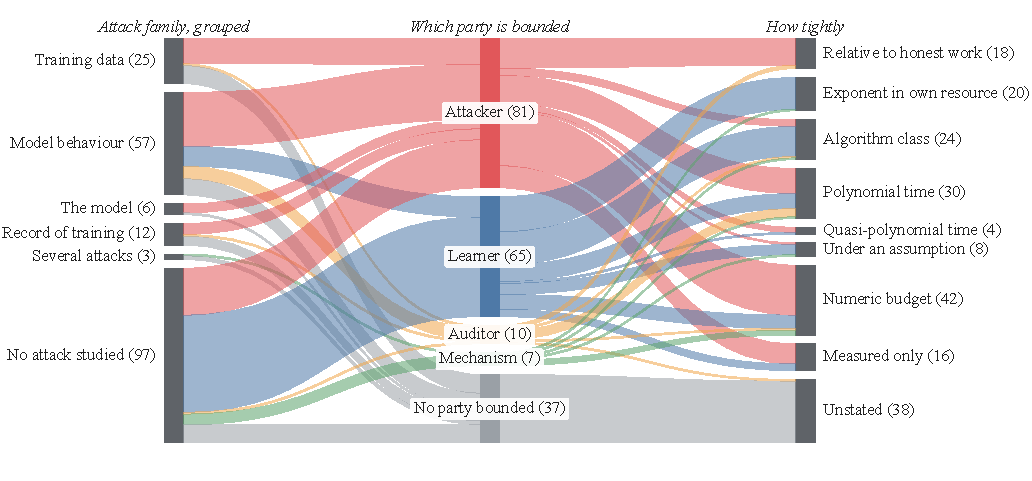
\includegraphics{figures/sankey-corpus}
\caption{The corpus of \NumSources{} works, flowing through what each work
attacks, which party it bounds, and how tightly. Band width is the number of
works and colour is the constrained party. The figure shows three of the
thirteen recorded fields. The supplementary material holds the full
classification. The first stage groups the attack families into five bands,
and the works that study no attack form the sixth.}
\label{fig:sankey}
\end{figure*}

Figure~\ref{fig:sankey} shows the corpus flowing through three of the recorded
fields. The supplementary material holds the full classification, on all
thirteen fields and with every work named by citation, and
Table~\ref{tab:worked} shows one work read through every field. Each finding
below names what is dense, what is empty, and what the emptiness means.

\begin{table}[t]
\centering
\small
\caption{One work read through every field: the sample complexity of membership
inference by Haghifam, Smith and Ullman \cite{HSU25}. The bound falls on the
attacker, in samples, relative to the samples the trainer used, and the quoted
sentence is the row's evidence.}
\label{tab:worked}
\begin{tabular}{@{}ll@{}}
\toprule
Field & Value \\
\midrule
target & train data \\
family & membership \\
phase & post hoc \\
access & weights \\
write & read only \\
frame & statistical \\
party & attacker \\
unit & samples \\
tightness & relative \\
baseline & absent \\
second party & samples \\
second notion & none \\
assessed & explicit \\
\midrule
\multicolumn{2}{@{}p{7.9cm}@{}}{Evidence, Theorem 1.1: ``every sample-based MIA
for the Gaussian mean estimation problem (Section 1.1) requires
$m \gtrsim n^2\rho^2 + n$ samples''.} \\
\bottomrule
\end{tabular}
\end{table}

\subsection{The field shares a vocabulary for access and phase}

Of the \NumAttackWorks{} works that study an attack, \AttackAccessNamed{} name
an access level, and they draw those values from one list of six: white box,
black box, confidence scores, hard labels, weights, gradients. Of those,
\AttackPostHoc{} attack a released model, \AttackTestTime{} attack a model at
test time, and \AttackTrainTime{} attack the training run. The five largest
cells of the phase-by-access table hold \PhaseAccessTopFive{} per cent of
these works, and works from different subfields fall in the same cells without
argument.
% claim: field-shares-access-vocabulary

We establish this before the other findings, because it shows the field can
agree on a threat-model dimension. The disagreement the rest of this section
documents is narrower than a general failure to standardize.

\subsection{Where it agrees on resources, it agrees on stating none}

The same works concentrate against the party each bounds and the unit it uses,
and where they concentrate is the finding. Table~\ref{tab:attack-party-unit}
gives the counts. The two largest cells hold the works that bound no party
(\AttackUnbound{}) and the works that bound the adversary by a perturbation
radius (\AttackPerturb{}), and the five largest hold
\PartyUnitTopFive{} per cent. Among the \NumAttackWorks{} attack works the
adversary itself is bounded in time in \AttackTimeAttacker{}, by a
perturbation radius in \AttackPerturb{}, in queries in
\AttackQueriesAttacker{}, in samples in
\AttackSamplesAttacker{}, and by a corruption fraction in \AttackCorrupt{}.

\begin{table}[t]
\centering
\small
\caption{The \NumAttackWorks{} works that study an attack, by the party their main claim bounds and the unit of that bound. The largest cell is no party in no unit.}
\label{tab:attack-party-unit}
\begin{tabular}{@{}lrrrrr@{}}
\toprule
Unit & Attacker & Learner & Auditor & Mechanism & None \\
\midrule
time & 17 & 3 & 7 &  &  \\
none &  &  &  &  & 27 \\
perturbation & 20 &  &  &  &  \\
queries & 9 & 1 &  &  &  \\
samples & 2 & 6 & 2 &  &  \\
corruption & 5 &  &  &  &  \\
algo class & 1 & 1 &  &  &  \\
privacy budget &  &  &  & 1 &  \\
circuit size & 1 &  &  &  &  \\
\bottomrule
\end{tabular}
\end{table}


The row for memory carries the finding. \AttackerMemory{} works bound an
adversary in memory, every one of them bounded-storage cryptography, and none
studies an attack on a learned model. The bounded-storage literature has spent
two decades on adversaries limited in space, and no work in this corpus
carries that restriction to an adversary attacking a model.
% claim: no-memory-bounded-adversary-attacks-a-model
% claim: most-formal-works-price-nobody

\subsection{The comparable form of bound is rare in attack papers}

A bound is comparable across papers when it relates one party's work to
another's, because only then can a reader ask whether one defence costs an
attacker more than another. \NumRelative{} of the \NumSources{} works state a
bound in that form, and Table~\ref{tab:relative} lists each with the relation
it states. \NumRelativeAttack{} of the \NumRelative{} study an attack: the
proof-of-learning requirement of Section~\ref{sec:problem-two}
\cite{JYCDTCP21}, a sample bound for membership inference \cite{HSU25}, a query
bound for adaptive data analysis \cite{HU14}, and three that price a filter, a
verifier or a forger against the work it audits or forges
\cite{BGGKRR26,NK26,ZCSL24}. The other twelve are cryptography with no machine
learning content.
% claim: two-party-bounds-rare-in-attack-papers

\begin{table*}[t]
\centering
\small
\caption{The \NumRelative{} works that state a bound as a relation between two parties' work. The first \NumRelativeAttack{} study an attack; the rest are cryptography with no machine learning content. Each relation is given in the source's own notation.}
\label{tab:relative}
\begin{tabular}{@{}lllp{2.2cm}p{7.4cm}@{}}
\toprule
Work & Attack & Bounded party, unit & Second party's unit & Relation as stated \\
\midrule
\cite{NK26} & evade audit & auditor, samples & samples & verifier sample complexity $O(\log k/\tau^2)$ against a prover's $\tilde\Theta(\sqrt{k})$ \\
\cite{BGGKRR26} & evade & auditor, time & time & every filter running in time $o(t^{\varepsilon})$ fails against a model running in time $t$ \\
\cite{HSU25} & membership & attacker, samples & samples & attacker needs $m \gtrsim n^2\rho^2 + n$ samples against a trainer's $n$ \\
\cite{HU14} & reconstruct & attacker, queries & samples & no efficient oracle holding $n$ samples answers $n^{3+o(1)}$ adaptive queries accurately \\
\cite{JYCDTCP21} & forge & attacker, time & time & $\mathbb{E}[C_A] \geq \mathbb{E}[C_T]$ for every spoofing strategy $A$ against honest training $T$ \\
\cite{ZCSL24} & evade audit & attacker, time & time & forging time $T(n)$ equal to the time $T(n)$ of retraining \\
\midrule
\cite{DQW22} & none & attacker, memory & memory & adversary memory $m = O(n^2)$ against honest parties holding $n$ bits \\
\cite{BRSV17} & none & attacker, time & time & no $O(t(n)^{1-\delta})$-time algorithm inverts a function computable in time $t(n)$ \\
\cite{GZ19} & none & attacker, memory & memory & adversary space $Cn^2$ against honest space $O(n)$ \\
\cite{BCEQ24} & none & attacker, memory & memory & key agreement with adversary space $a \gg s^2$ against honest space $s$ needs one-way functions \\
\cite{ACMS23} & none & attacker, queries & queries & adversary $n^{K/(K-1)}$ oracle queries against honest parties' $n$ \\
\cite{BCS24} & none & attacker, time & time & adversary time $O(n^{2-\varepsilon})$ against honest time $n$ \\
\cite{BC22} & none & attacker, circuit size & circuit size & no circuit of size $o(|f|^{1+\delta})$ inverts $f$ with probability above $\varepsilon$ \\
\cite{BM09} & none & attacker, queries & queries & adversary $O(n^2)$ oracle queries against honest parties' $n$ \\
\cite{BGHKP24} & none & attacker, time & time & adversarial power $T^{1-\varepsilon}$ against honest power $T$ \\
\cite{LLW19} & none & attacker, time & time & honest evaluation in time $T(n)^{1-\delta}$, no adversary of time $T(n)$ inverts \\
\cite{GM24} & none & attacker, circuit depth & circuit depth & adversary parallel time below $k \cdot t_A(\lambda)$ against $k$ honest sequential evaluations \\
\cite{DQW23} & none & attacker, memory & memory & adversary memory $m$ up to $2^{O(n)}$ against honest memory $n$ \\
\bottomrule
\end{tabular}
\end{table*}


A bound written as an exponent is a different object. A neural scaling law and
a sample-complexity threshold are exponents in one party's own resource, with
no second party anywhere, and \NumExponent{} works in this corpus are of that
kind. An exponent in one party's resource says how that party's cost grows. A
relation between two parties' work says what the second must spend to defeat
the first, and only the second form places two results on one scale.

The attack literature uses neither form often. Of the \NumAttackWorks{} attack
works, \AttackBudget{} state a budget, meaning a numeric allowance such as a
perturbation radius that carries no relation to anything the defender does.
\AttackUnstated{} state no tightness at all. \AttackPoly{} use the binary
polynomial-time quantifier, \AttackMeasured{} report a measurement with no
definitional standing, and \AttackClass{} name a restricted algorithm class.
% claim: attack-bounds-limit-change-not-spend

\subsection{The attack literature prices nobody more often, and how much more is uncertain}

\AttackUnbound{} of the \NumAttackWorks{} works studying an attack bound no
party in any resource. \TheoryUnbound{} of the \NumTheoryWorks{} works with no
attack family do. The rates are \RateAttack{} and \RateOther{} per cent, a
ratio of about \RatioUnbound{}, with a \ConfLevel{} per cent interval on the
difference of \DiffLo{} to \DiffHi{} percentage points.

Who enters each half moves that comparison, and the sensitivity runs against
the finding. Systematizations, position papers and evaluation
critiques dominate the unbounded attack works. They enter through the third
reading of our inclusion test and bound nobody because their claims concern
practice and not an adversary. Restricting both halves to works whose main
claim is a theorem and not a measurement gives \ThmAttackUnbound{} of
\ThmAttack{} against
\ThmOtherUnbound{} of \ThmOther{}. The ratio is similar, near \ThmRatio{}, and
the interval on the difference then runs from \ThmDiffLo{} to \ThmDiffHi{}
percentage points and includes zero.

We therefore state the direction and not the size. The attack literature
bounds no party more often than the cryptography and learning-theory
literature does, and this corpus leaves the margin open. Establishing it would
need a corpus assembled by sampling a frame, and not the working bibliography
we used here.
% claim: attack-works-price-nobody-more-often
% claim: margin-direction-only
% claim: corpus-is-a-working-bibliography

\subsection{Works that hold a quantity their framing does not carry}

Our classification records, separately from how tightly a work states its
bound, whether the work treats that bound as its object or leaves it a side
condition. Across the corpus the two agree \AssessedPredictable{} per cent of
the time, which makes the \NearMiss{} works where they disagree worth listing.
Table~\ref{tab:nearmiss} names each and the quantity it holds.
% claim: classification-of-two-hundred-works

\begin{table*}[t]
\centering
\small
\caption{The \NearMiss{} works whose stated tightness and treatment of the bound disagree. Kind records what the quantity is: \NearMissAdv{} hold an adversary's or auditor's cost, \NearMissTrain{} a training cost, and \NearMissCap{} a capability or a mechanism parameter.}
\label{tab:nearmiss}
\begin{tabular}{@{}lp{3.2cm}p{2.4cm}p{6.6cm}p{2.7cm}@{}}
\toprule
Work & Kind & Tightness, treatment & Quantity held & Where \\
\midrule
\cite{DKLP22} & adversary's cost & measured, explicit & attacker compute raised up to a hundredfold by a proof-of-work puzzle, measured & abstract \\
\cite{NCM25} & adversary's cost & budget, implicit & a $q$-query adversary, fixed as a definition and not studied & admissible-adversary definition \\
\cite{BGGKRR26} & adversary's cost & relative, implicit & filter time $o(t^{\varepsilon})$ against model time $t$, a side condition of Theorem 1 & Theorem 1 \\
\cite{ZDKT25} & adversary's cost & unstated, implicit & the cost of retraining a large model to sample the null, assessed and never stated as a bound & abstract \\
\cite{ZFWCSXZ26} & adversary's cost & budget, implicit & a dishonest prover's cost per epoch, assumed to be zero & Section 3.3 \\
\cite{DJYWWMNL26} & adversary's cost & measured, explicit & forging cost of 1.1 to 4 times honest proof generation, measured & evaluation \\
\cite{FK24} & adversary's cost & budget, implicit & the number of queries left to the adversary, a game parameter not studied & security game \\
\cite{CGZ24} & adversary's cost & measured, explicit & one query per output token to remove the watermark, and a cost ratio in dollars & Theorem 11 and evaluation \\
\cite{ZCSL24} & adversary's cost & relative, implicit & forging time equal to retraining time, reported beside a validity criterion that ignores it & Proposition 4.5 \\
\midrule
\cite{HBEORGATS24} & training cost & measured, explicit & the compute needed for a fixed loss, halving every eight months, measured & abstract \\
\cite{SGSGM22} & training cost & measured, explicit & the exponent of a scaling law in data, measured & experiments \\
\cite{BAP25} & training cost & measured, explicit & the exponent of a scaling law, measured & experiments \\
\cite{BEGKMZ22} & training cost & measured, explicit & steps to convergence as a power law $t_c \propto n^{\alpha k}$, measured & experiments \\
\cite{BBHS22} & training cost & budget, implicit & the learner's calls to an empirical risk minimization oracle & Theorem 3.1 \\
\midrule
\cite{CGBSHC22} & capability or mechanism & budget, implicit & a norm bound on the perturbation, fixed as a definition and not studied & attack definition \\
\cite{SAHBS26} & capability or mechanism & budget, implicit & the mechanism's privacy budget, with the adversary left unconstrained & main theorem \\
\cite{YHGA25} & capability or mechanism & class, implicit & the class of local unlearning algorithms, a definition & definition of a local algorithm \\
\cite{CAPBRTGMK19} & capability or mechanism & budget, implicit & the perturbation budget fixed as a definition, while attacker compute is rejected in the text & Sections 2.2.2 and 4.8 \\
\cite{RT24} & capability or mechanism & measured, explicit & a corruption fraction of half a per cent of preference data, measured & evaluation \\
\bottomrule
\end{tabular}
\end{table*}


\NearMissA{} of them state a bound in definitional form and treat something else
as the thing being studied. The filtering impossibility is the clearest. Its
theorem turns on the filter running no faster than the model it audits, which
relates two parties' compute, and the paper states it as a side
condition and not as the quantity the result is about \cite{BGGKRR26}. The
evaluation guidance that declines attacker compute as a threat-model parameter
nonetheless fixes a perturbation radius and reasons about gradient-step counts
\cite{CAPBRTGMK19}. A proof-of-learning follow-up prices a forgery against
honest training and leaves the ratio unparameterized \cite{ZFWCSXZ26}.

\NearMissB{} run the other way, treating a cost deliberately while stating it
only as a measurement. Dziedzic et al.\ calibrate a proof-of-work puzzle to
how much a client has already extracted, which prices an adversary in compute,
with no definition and no theorem attached \cite{DKLP22}. Three of the
\NearMissB{} are scaling and learning-dynamics results whose measured quantity
is a training cost that the scaling literature already names
\cite{SGSGM22,BAP25,BEGKMZ22}.

The remaining one states no tightness at all while plainly assessing a
resource. The position that membership inference cannot establish training-set
membership rests, in its second and independent argument, on the cost of
sampling a null hypothesis that would require training new large models
\cite{ZDKT25}.

The \NearMiss{} works are three phenomena, and Table~\ref{tab:nearmiss} says
which is which. \NearMissAdv{} hold an adversary's or an auditor's cost, and
those are where the quantity this survey is about already exists in the
literature without a name. \NearMissTrain{} hold a training cost.
\NearMissCap{} hold a capability or a mechanism parameter that the same
mechanical test flags, because the work states it as a definition and studies
something else.
% claim: near-miss-works-hold-unnamed-adversary-price

\subsection{Baselines in the attack literature}

An advantage is a success rate minus what public knowledge alone achieves, so
a work that defines adversary success without naming that reference reports a
number with nothing to subtract. \BaselineNA{} of the \NumSources{} works
define no adversary success criterion, which is the correct answer for a
learning theory result with no adversary in it. Among the \NumAttackWorks{}
works that study an attack, \BaselineCrit{} define what success means, and of
those
\BaselineStated{} name a baseline while \BaselineAbsent{} omit one.
% claim: baselines-absent-in-attack-papers

Re-reading every row under the narrower definition changed \BaselineChanged{}
values, and the errors had four shapes, each a plausible mistake. A reader
took an information-theoretic optimum for a baseline, when it describes the
best any algorithm could do and not what an adversary without access achieves.
A reader took a previously published accuracy number for one, when it
describes a different attack. A reader took the cost of an alternative
algorithm for one. And in an unforgeability game a reader took the raw success
tolerance for a coin flip, when a search game has no coin-flip structure.
